\chapter{Section 2:  Seasons and Calendars across cultures}
The purely qualitative methods, results, and interpretive discussion.

\section{Methods}
%Qualitative; snowball interview recruitment with three 'seeds' (Yolngu, UCA, Science).
%Reflecting on results, it's more complex than I first thought.

I initially planned to gather qualitative data on the Yolngu seasonal calendar
from published resources and interviews with Yolngu people.
Over the course of my research, several unforseen approaches have also proved important.

I conducted a series of informal, semistructured interviews centered around discussion of seasons and climate.
Recruitment was primarily by a `snowball' pattern, where participants were asked to
suggest further potential participants.
See \ref{Ethics} for details of the human ethics approval.
The main `seeds' of this pattern were personal contacts, some Yolngu and some non-indigenous
people who have spent decades living and working in remote communities.
I followed several disconnected threads such as the \citet{CSIROcals} project,
which helped to clarify and test my interpretation of the interviews.

I rely on four sources of knowledge and context for the Yolngu seasons, in rough order of importance:

\begin{itemize}
\item Interview with Yolngu people form the basis of my qualitative research, and
        are the definitive source of information about Yolngu seasons.
\item Interviews and discussion with non-indigenous researchers or teachers experienced
        in remote communities help contextualise this knowledge, and warned of
        common misinterpretations - as well as pointing out nuance.
\item Published literature, particularly around cross-cultural research \citep[eg.][]{smith1999},
        Australian indigenous seasons \citep[eg.][]{prober2011,oconnor2010}, and Yolngu
        seasons directly \citep{davis1989}.
\item Grey literature, such as posters produced for use in remote schools, workbooks
        for cross-cultural teacher training, etc.
\end{itemize}

The literature contextualises and informs the interviews, and suggested many fruitful
directions for direct questions or later searches for documents.


Following the interviews, I also engaged in substantial reflection on the nature of
my questions and the ambiguity of the responses and data I collected.

all in english
what is a season
what is a calendar
there is no ``the'' yolngu calendar - varies spatially, multiple seasonal calendars for different temporal scales with varied purposes
`simple fact-finding' really isn't!



\section{Results and Discussion}

The qualitative results are fall into four subsections.
First, a review of the literature relevant to Yolngu seasons, including unpublished documents.
Second, personal reflections following my interviews, as above.
Third, a summary of the emergent themes in my interviews.
Fourth and finally, a Yolngu seasonal calendar drawn from interiew responses and aligned with \citet{davis1989}.




`Calendar' and `season' are not concepts that translate directly across cultures. 

Discuss how I realised this, by re-listening to recordings, and that I was expecting something unforeseen (but not like this!).  

Yolngu participants discussed three levels of seasons:
\begin{itemize}
\item A Wet-Dry seasonality, based on the monsoon winds;
\item A six-season calendar defined primarily by wind, rain, and temperature; and
\item Phenological seasons, where ecological events signal appropriate activities.
\end{itemize}

Of these, the wet/dry monsoon seasonal cycle is most likely familiar to non-indigenous people,
especially in the tropics.  Yolngu participants emphasised that these seasons
are \textit{not} recognised by rainfall, but rather the direction of prevailing winds.
Interestingly, this mirrors the meteorological definition of monsoon, where rainfall is less important than
the location of the intertropical convergence zone and consequent direction of prevailing wind.




\ref{fig:ngangi-seasons} shows 

Use TRaCK poster to highlight the six and many seasons (each box a microseason).

The two are <give some detail or quotes>.
The six are <>.

Completeness of the many is out of scope, but <examples>.  

For the remainder of this thesis I'll focus on the six, which best facilitates knowledge synthesis.


\begin{figure}[h]
    \centering
    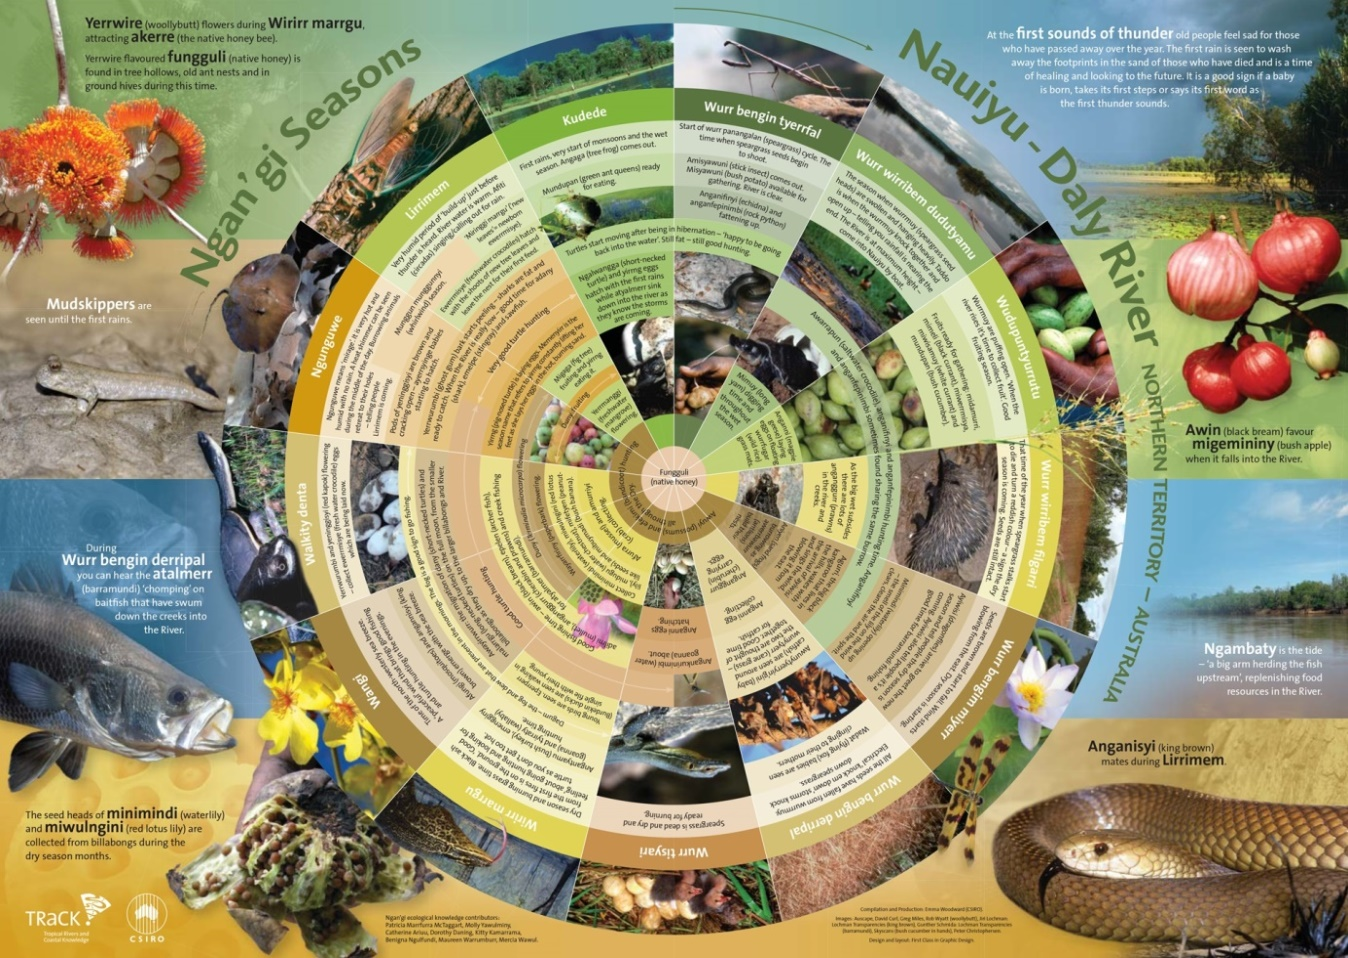
\includegraphics[width=0.8\textwidth]{ngangi-calendar.jpg}
    \caption{An indigenous seasonal calendar, for Ngan'gi seasons \citep{CSIROcals}}
    \label{fig:ngangi-seasons}
\end{figure}

